\documentclass[11pt, aspectratio=169]{beamer}
\usetheme{Thesis}

\usepackage[latin1]{inputenc}
\usepackage{amsmath,amsfonts,amssymb}
\usepackage{graphics}
\usepackage{graphicx}
\usepackage{xcolor}
\usepackage{setspace}


\usepackage{tikz}
\usetikzlibrary{arrows,shapes,shadows,calc}

\setbeamertemplate{itemize/enumerate body begin}{\small}
\setbeamertemplate{itemize/enumerate subbody begin}{\footnotesize}

\setlength{\itemsep}{1ex}




%%%%%%%%%%%%%%%%%%%%%%%%%%%%%%%%%%%%%%%%%%%%%%%
% COLOR Command
\newcommand{\myemph}[1]{\emph{\color{emph@Thesis}#1}}
\newcommand{\mytitle}[1]{\textbf{\color{emph@Thesis}#1}}
\newcommand{\myblue}[1]{{\color{blue@Thesis}#1}}
\newcommand{\myred}[1]{{\color{red@Thesis}#1}}
%%%%%%%%%%%%%%%%%%%%%%%%%%%%%%%%%%%%%%%%%%%%%%%

\title[Control of an autonomous aerodynamic airshield]
  {\Large Control of an autonomous aerodynamic airshield \\
for training Olympics 100m sprint athletes}
\author[Giulia Cutini]{Giulia Cutini}
\institute[University of Bologna]{}
\date{\today}



\graphicspath{{figs/}}


\begin{document}
\footnotesize

%%%%%%%%%%%%%%%%%%%%%%%%%%%%%%%%%%%%%%%%%%%%%%%%%%%%%%%%%%%%%%%%%%%%%%%%%%%%%%%%
%%%%%%%%%%%%%%%%%%%%%%%%%%%%%%%%%%%%%%%%%%%%%%%%%%%%%%%%%%%%%%%%%%%%%%%%%%%%%%%%

\begin{frame}[plain,noframenumbering,t]
\centering

\vspace{0.8cm}
\begin{columns}
\begin{column}{1.1\textwidth}
\centering \footnotesize
\textsc{Alma Mater Studiorum Universit\`{a} di Bologna}\\
\textsc{Department of Electrical, Electronic and Information Engineering}
\\
\vspace{0.2cm}
\textsc{Master's Degree in Automation Engineering}
\end{column}
\end{columns}

\vspace{0.5cm}

\textcolor{blue@Thesis}{\Large \bf \inserttitle}

\vspace{1cm}

\begin{columns}[t]
\begin{column}{0.5\textwidth}
	\myemph{Candidate:}
	
	\hspace{0.5cm} Giulia Cutini
\end{column}

\begin{column}{0.4\textwidth}
	\myemph{Advisor:}
	
		\hspace{0.5cm} Prof.~Giuseppe Notarstefano
		
		\vspace{.4cm}
		\myemph{Co-Advisors:}
	
		\hspace{0.5cm} Prof.~Melanie Zeilinger \\
		\hspace{0.5cm} Dr.~Andrea Carron \\
		\hspace{0.5cm} Ing.~Lorenzo Sforni
\end{column}
	
\end{columns}

\begin{tikzpicture}[remember picture,overlay]
\node[anchor=south west,inner sep=0pt] at (current page.south west) {
	\hspace{1cm} 
\includegraphics[height=1.5cm]{Logo_unibo}
};
\node[anchor=south east,inner sep=0pt] at (current page.south east) {
	
\includegraphics[height=0.8cm]{Logo_ETH}  \hspace{1cm} 
};
\end{tikzpicture}

\vspace{0.5cm}
\begin{center}
\scriptsize
  \textcolor{emph@Thesis}{Bologna, 18 March 2024}
\end{center}


\end{frame}

%%%%%%%%%%%%%%%%%%%%%%%%%%%%%%%%%%%%%%%%%%%%%%%%%%%%%%%%%%%%%%%%%%%%%%%%%%%%%%%%
%%%%%%%%%%%%%%%%%%%%%%%%%%%%%%%%%%%%%%%%%%%%%%%%%%%%%%%%%%%%%%%%%%%%%%%%%%%%%%%%

\begin{frame}
\frametitle{Table of Contents}
\begin{itemize}
	\item[$\blacktriangleright$]<1-> Introduction
		\begin{itemize}
			\small
			\item[$\triangleright$]<1-> Motivations
			\item[$\triangleright$]<1-> Contributions
		\end{itemize}
	\item[$\blacktriangleright$]<2-> Modeling of the go-kart with the airshield attached
	\item[$\blacktriangleright$]<3-> Control design
		\begin{itemize}
		\small
			\item[$\triangleright$]<3-> Gain Scheduling Linear Quadratic Regulator
			\item[$\triangleright$]<3-> Model Predictive Control
			\item[$\triangleright$]<3-> Offset-free Model Predictive Control
		\end{itemize}
	\item[$\blacktriangleright$]<4-> Simulation test and numerical controllers comparison
	\item[$\blacktriangleright$]<5-> Hardware-in-the-loop tests
\end{itemize}
\end{frame}


%%%%%%%%%%%%%%%%%%%%%%%%%%%%%%%%%%%%%%%%%%%%%%%%%%%%%%%%%%%%%%%%%%%%%%%%%%%%%%%
%%%%%%%%%%%%%%%%%%%%%%%%%%%%%%%%%%%%%%%%%%%%%%%%%%%%%%%%%%%%%%%%%%%%%%%%%%%%%%%

\begin{frame}[t]
\frametitle{Introduction}
\vspace{0.1cm}
\textcolor{emph@Thesis}{\textbf{\small{Motivations}}} \\
\vspace{0.1cm}
In athletics the \textbf{overspeed training} makes possible to enhance the competition performances.

\setstretch{1.3}
It can be achieved by isolating the runner from the air resistance using an \textbf{airshield}.

\begin{columns}
\hspace{0.2cm}
\begin{column}{0.4\textwidth}
\setstretch{0.5}
The usage of an \textbf{autonomous go-kart}:
	\begin{itemize}
		\item[$\blacktriangleright$] simpler maneuvering
		\item[$\blacktriangleright$] safer maneuvering
	\end{itemize}
\end{column}
\begin{column}{0.6\textwidth}
	\begin{center}
  		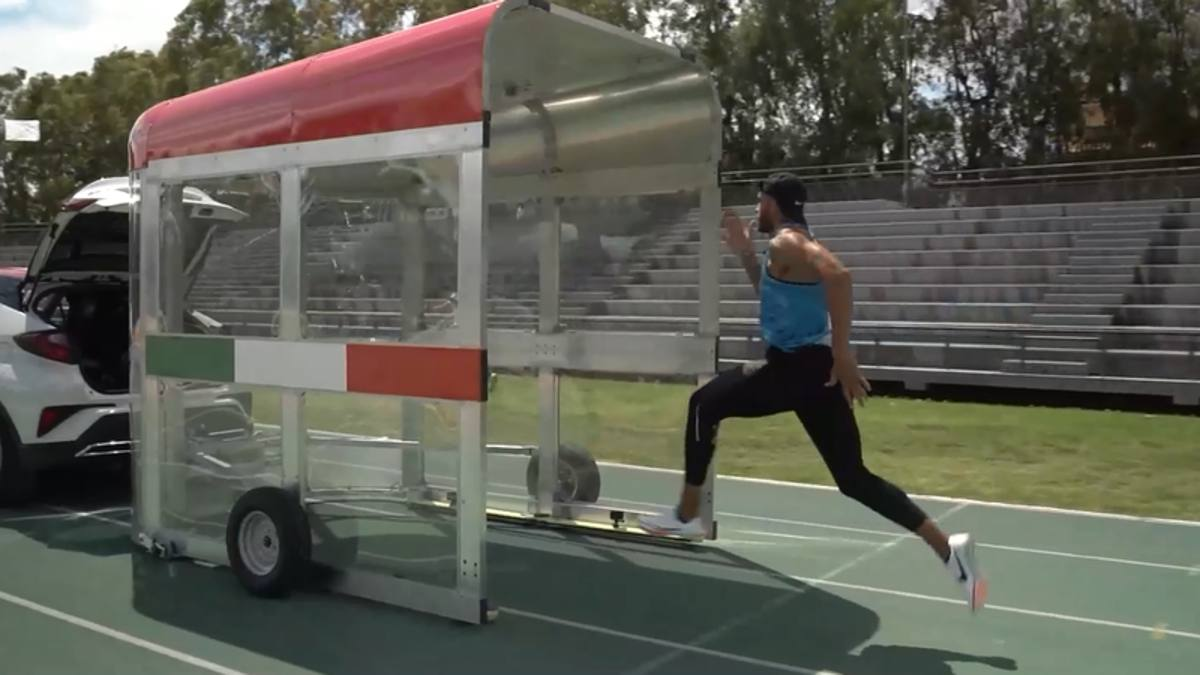
\includegraphics[width=0.48\textwidth]{Jacobs} 
		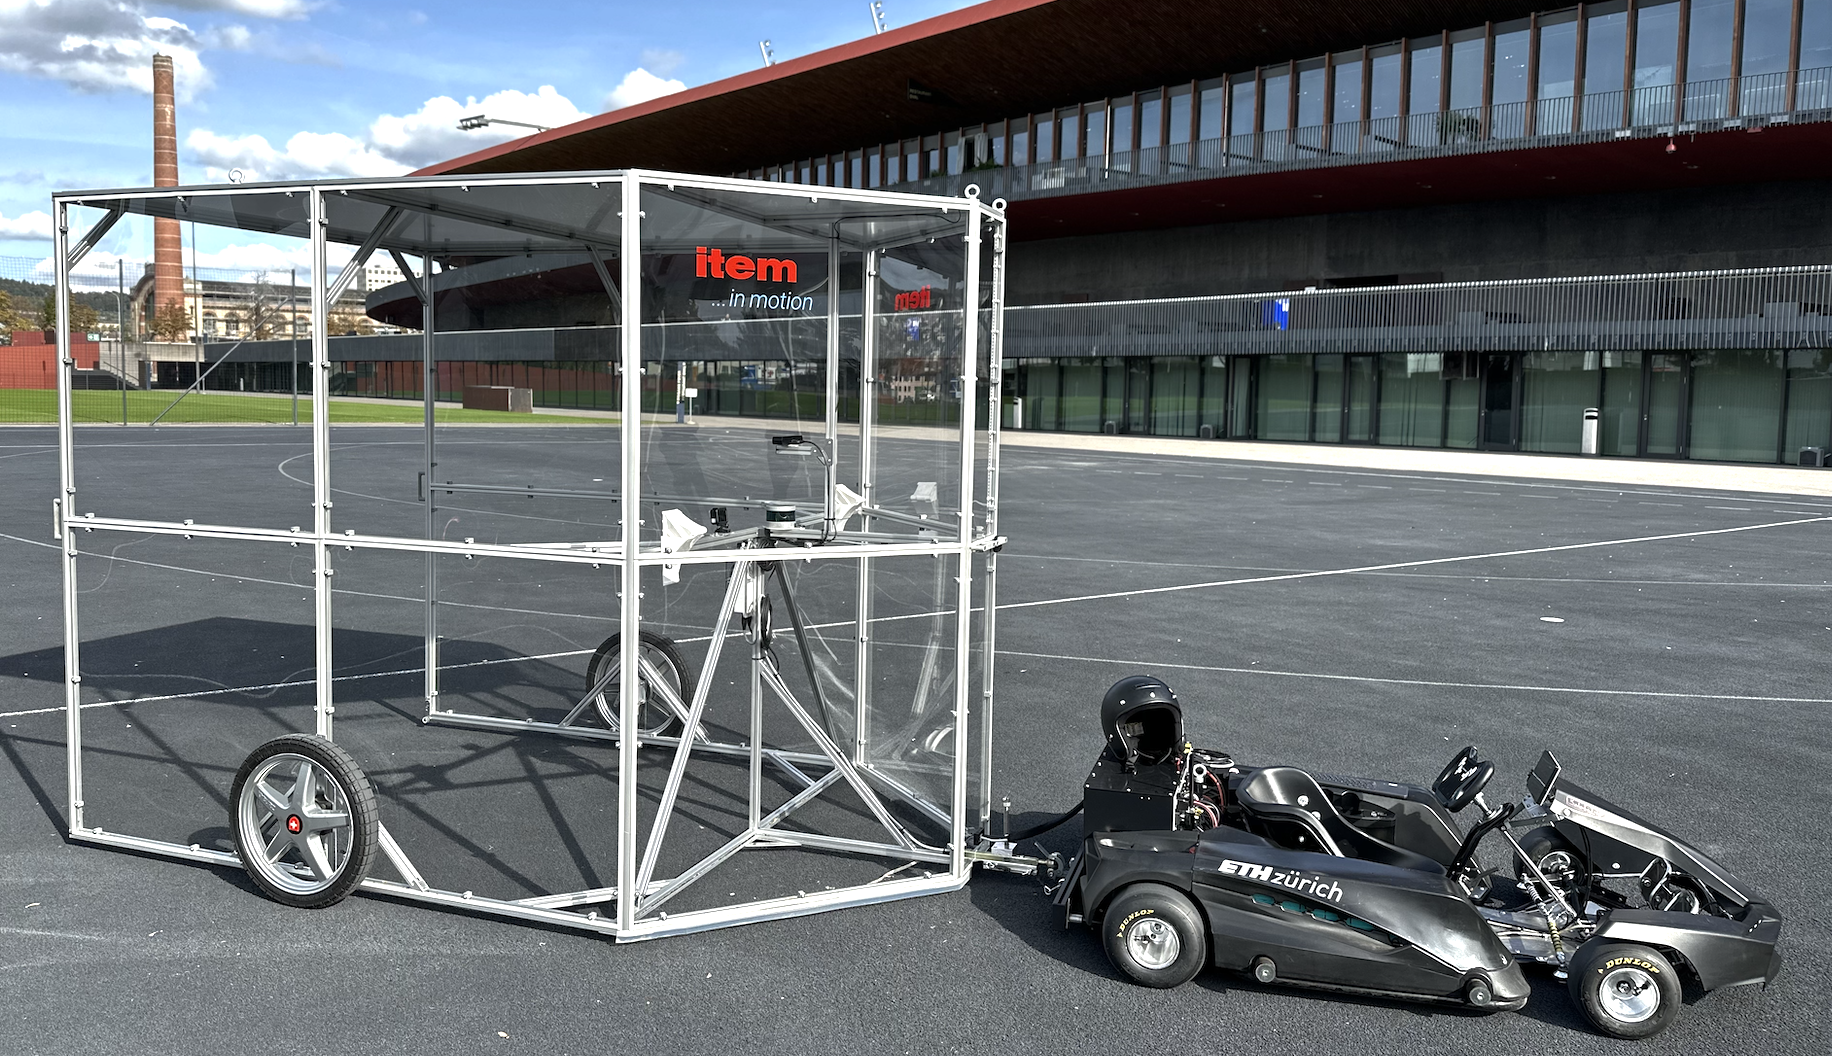
\includegraphics[width=0.47\textwidth]{Windshield} 
	\end{center}
\end{column}
\end{columns}
\vspace{0.1cm}

\vspace{0.1cm}
\textcolor{emph@Thesis}{\textbf{\small{Contributions}}} \\
\vspace{0.1cm}

\end{frame}




\section{Modeling of the go-kart with the airshield attached}
\begin{frame}[t]
\frametitle{Modeling of the go-kart with the aishield attached}
\end{frame}

\section{Control design}
\subsection{Linear Quadratic Regulator}
\begin{frame}[t]
\frametitle{Gain Scheduling Linear Quadratic Regulator}
\end{frame}


\subsection{Model Predictive Control}
\begin{frame}
\frametitle{Model Predictive Control}
\end{frame}


\subsection{Offset-free Model Predictive Control}
\begin{frame}
\frametitle{Offset-free Model Predictive Control}
\end{frame}

\section{Simulation tests and Controllers comparison}
\begin{frame}
\frametitle{Simulation tests and Controllers comparison}
\end{frame}

\section{Hardware-in-the-loop tests}
\begin{frame}
\frametitle{Hardware-in-the-loop tests}
\end{frame}
\end{document}

\begin{columns}
\begin{column}{0.5\linewidth}


Some text
%
\begin{itemize}
\item Bullet 1
\item Bullet 2
\item Bullet 3
\end{itemize}

\end{column}
%
\begin{column}{0.5\textwidth}

\begin{center}
  \includegraphics[scale=1]{example_figure.pdf}
\end{center}

\end{column} 
\end{columns}

\vspace{1cm}
An equation
\begin{align*}
\dot{x} = f(x,u)
\end{align*}


